\documentclass[a4paper]{book}
\usepackage{a4wide}
\usepackage{makeidx}
\usepackage{fancyhdr}
\usepackage{graphicx}
\usepackage{multicol}
\usepackage{float}
\usepackage{textcomp}
\usepackage{alltt}
\usepackage{doxygen}
\makeindex
\setcounter{tocdepth}{1}
\renewcommand{\footrulewidth}{0.4pt}
\begin{document}
\begin{titlepage}
\vspace*{7cm}
\begin{center}
{\Large LABVIEW2LCIO Reference Manual\\[1ex]\large 1.0.0 }\\
\vspace*{1cm}
{\large Generated by Doxygen 1.4.7}\\
\vspace*{0.5cm}
{\small Fri Nov 14 17:58:38 2014}\\
\end{center}
\end{titlepage}
\clearemptydoublepage
\pagenumbering{roman}
\tableofcontents
\clearemptydoublepage
\pagenumbering{arabic}
\chapter{LABVIEW2LCIO Directory Hierarchy}
\section{Directories}
This directory hierarchy is sorted roughly, but not completely, alphabetically:\begin{DoxyCompactList}
\item \contentsline{section}{calice\_\-reco}{\pageref{dir_f98b43a53f5533225f05987ae358305b}}{}
\begin{DoxyCompactList}
\item \contentsline{section}{recoSiPM}{\pageref{dir_01780ac29724157a4922dcd586d6082b}}{}
\begin{DoxyCompactList}
\item \contentsline{section}{include}{\pageref{dir_c3d352f5158c78b0c23f5f807db2ef1c}}{}
\item \contentsline{section}{src}{\pageref{dir_1f1ceb4cb990831dc6e091a4a09bb7bd}}{}
\end{DoxyCompactList}
\end{DoxyCompactList}
\end{DoxyCompactList}

\chapter{LABVIEW2LCIO Namespace Index}
\section{Namespace List}
Here is a list of all documented namespaces with brief descriptions:\begin{DoxyCompactList}
\item\contentsline{section}{{\bf CALICE} (Store strings in LCGenericObjects )}{\pageref{namespaceCALICE}}{}
\item\contentsline{section}{{\bf marlin} (The namespace \doxyref{CALICE}{p.}{namespaceCALICE} contains calice specific software needed for the processing of \doxyref{CALICE}{p.}{namespaceCALICE} data including the interface classes to the \doxyref{CALICE}{p.}{namespaceCALICE} Raw Data and convenient MARLIN processors )}{\pageref{namespacemarlin}}{}
\end{DoxyCompactList}

\chapter{LABVIEW2LCIO Data Structure Index}
\section{LABVIEW2LCIO Data Structures}
Here are the data structures with brief descriptions:\begin{CompactList}
\item\contentsline{section}{\bf{CALICE::Event\-Checker} (Class to process Labview raw )}{\pageref{classCALICE_1_1EventChecker}}{}
\item\contentsline{section}{\bf{CALICE::HBUTemperature\-Block} (Class for the Labview Data as acquired by the AHCAL Labview )}{\pageref{classCALICE_1_1HBUTemperatureBlock}}{}
\item\contentsline{section}{\bf{CALICE::Labview\-Block} (Class for the Labview Data as acquired by the AHCAL Labview )}{\pageref{classCALICE_1_1LabviewBlock}}{}
\item\contentsline{section}{\bf{CALICE::Labview\-Block2} (Class for the Labview Data as acquired by the AHCAL Labview )}{\pageref{classCALICE_1_1LabviewBlock2}}{}
\item\contentsline{section}{\bf{marlin::Labview\-Converter} (Processor for reading the AHCAL Labview asscii files )}{\pageref{classmarlin_1_1LabviewConverter}}{}
\item\contentsline{section}{\bf{marlin::Labview\-Converter2} (Processor for reading the AHCAL Labview asscii files )}{\pageref{classmarlin_1_1LabviewConverter2}}{}
\item\contentsline{section}{\bf{marlin::Labview\-Converter2::raw\-Data} (The labview data format )}{\pageref{structmarlin_1_1LabviewConverter2_1_1rawData}}{}
\item\contentsline{section}{\bf{LConverter} }{\pageref{classLConverter}}{}
\item\contentsline{section}{\bf{CALICE::Root\-Tree\-Generator} (Class to process Labview raw )}{\pageref{classCALICE_1_1RootTreeGenerator}}{}
\item\contentsline{section}{\bf{CALICE::Root\-Tree\-Generator2} (Class to process Labview raw )}{\pageref{classCALICE_1_1RootTreeGenerator2}}{}
\item\contentsline{section}{\bf{marlin::Root\-Write\-Engine} (Abstract base class of callback classes for the Root\-Tree\-Write processor Abstract interface for a Root\-Tree\-Writer-engine )}{\pageref{classmarlin_1_1RootWriteEngine}}{}
\item\contentsline{section}{\bf{CALICE::Temp\-Sensor\-Block} (Class for the Labview Data as acquired by the AHCAL Labview )}{\pageref{classCALICE_1_1TempSensorBlock}}{}
\end{CompactList}

\chapter{LABVIEW2LCIO Page Index}
\section{LABVIEW2LCIO Related Pages}
Here is a list of all related documentation pages:\begin{CompactList}
\item \contentsline{section}{Todo List}{\pageref{todo}}{}

\end{CompactList}

\chapter{LABVIEW2LCIO Directory Documentation}
\section{/afs/desy.de/group/flc/pool/ebrianne/Projects/AHCAL/Reco\_\-soft\_\-CALICE/labview-converter/raw2lcio/include/ Directory Reference}
\label{dir_7e1ef05074d24d5c983464385fc8f8e7}\index{/afs/desy.de/group/flc/pool/ebrianne/Projects/AHCAL/Reco_soft_CALICE/labview-converter/raw2lcio/include/ Directory Reference@{/afs/desy.de/group/flc/pool/ebrianne/Projects/AHCAL/Reco\_\-soft\_\-CALICE/labview-converter/raw2lcio/include/ Directory Reference}}
\subsection*{Files}
\begin{CompactItemize}
\item 
file \textbf{Event\-Checker.hh}
\item 
file \textbf{HBUtemperature\-Block.hh}
\item 
file \textbf{Labview\-Block.hh}
\item 
file \textbf{Labview\-Block2.hh}
\item 
file \textbf{Labview\-Converter.hh}
\item 
file \textbf{Labview\-Converter2.hh}
\item 
file \textbf{LConverter.hh}
\item 
file \textbf{Root\-Tree\-Generator.hh}
\item 
file \textbf{Root\-Tree\-Generator2.hh}
\item 
file \textbf{Root\-Write\-Engine.hh}
\item 
file \textbf{Temp\-Sensor\-Block.hh}
\end{CompactItemize}

\section{/afs/desy.de/group/flc/pool/ebrianne/Projects/AHCAL/Reco\_\-soft\_\-CALICE/labview-converter/ Directory Reference}
\label{dir_f1b7cdcb1096f5f7a79309d2e7623073}\index{/afs/desy.de/group/flc/pool/ebrianne/Projects/AHCAL/Reco_soft_CALICE/labview-converter/ Directory Reference@{/afs/desy.de/group/flc/pool/ebrianne/Projects/AHCAL/Reco\_\-soft\_\-CALICE/labview-converter/ Directory Reference}}
\subsection*{Directories}
\begin{CompactItemize}
\item 
directory \bf{raw2lcio}
\end{CompactItemize}

\section{/afs/desy.de/group/flc/pool/ebrianne/Projects/AHCAL/Reco\_\-soft\_\-CALICE/labview-converter/raw2lcio/ Directory Reference}
\label{dir_5db2edf70535c52601f3c3ef5e1c406f}\index{/afs/desy.de/group/flc/pool/ebrianne/Projects/AHCAL/Reco_soft_CALICE/labview-converter/raw2lcio/ Directory Reference@{/afs/desy.de/group/flc/pool/ebrianne/Projects/AHCAL/Reco\_\-soft\_\-CALICE/labview-converter/raw2lcio/ Directory Reference}}
\subsection*{Directories}
\begin{CompactItemize}
\item 
directory \bf{include}
\item 
directory \bf{src}
\end{CompactItemize}

\section{/afs/desy.de/group/flc/pool/ebrianne/Projects/AHCAL/Reco\_\-soft\_\-CALICE/labview-converter/raw2lcio/src/ Directory Reference}
\label{dir_d85041cf67ee28c7f5693b4af2f90777}\index{/afs/desy.de/group/flc/pool/ebrianne/Projects/AHCAL/Reco_soft_CALICE/labview-converter/raw2lcio/src/ Directory Reference@{/afs/desy.de/group/flc/pool/ebrianne/Projects/AHCAL/Reco\_\-soft\_\-CALICE/labview-converter/raw2lcio/src/ Directory Reference}}
\subsection*{Files}
\begin{CompactItemize}
\item 
file \textbf{Event\-Checker.cc}
\item 
file \textbf{Labview\-Converter.cc}
\item 
file \textbf{Labview\-Converter2.cc}
\item 
file \textbf{Root\-Tree\-Generator.cc}
\item 
file \textbf{Root\-Tree\-Generator2.cc}
\item 
file \textbf{Root\-Tree\-Generator3.cc}
\end{CompactItemize}

\chapter{LABVIEW2LCIO Namespace Documentation}
\section{CALICE Namespace Reference}
\label{namespaceCALICE}\index{CALICE@{CALICE}}


\subsection*{Data Structures}
\begin{CompactItemize}
\item 
class \bf{Event\-Checker}
\begin{CompactList}\small\item\em Class to process Labview raw. \item\end{CompactList}\item 
class \bf{HBUTemperature\-Block}
\begin{CompactList}\small\item\em Class for the Labview Data as acquired by the AHCAL Labview. \item\end{CompactList}\item 
class \bf{Labview\-Block}
\begin{CompactList}\small\item\em Class for the Labview Data as acquired by the AHCAL Labview. \item\end{CompactList}\item 
class \bf{Labview\-Block2}
\begin{CompactList}\small\item\em Class for the Labview Data as acquired by the AHCAL Labview. \item\end{CompactList}\item 
class \bf{Root\-Tree\-Generator}
\begin{CompactList}\small\item\em Class to process Labview raw. \item\end{CompactList}\item 
class \bf{Root\-Tree\-Generator2}
\begin{CompactList}\small\item\em Class to process Labview raw. \item\end{CompactList}\item 
class \bf{Root\-Tree\-Generator3}
\begin{CompactList}\small\item\em Class to process Labview raw. \item\end{CompactList}\item 
class \bf{Temp\-Sensor\-Block}
\begin{CompactList}\small\item\em Class for the Labview Data as acquired by the AHCAL Labview. \item\end{CompactList}\item 
class \bf{Temp\-Sensor\-Block2}
\begin{CompactList}\small\item\em Class for the Labview Data as acquired by the AHCAL Labview. \item\end{CompactList}\item 
class \bf{Temp\-Sensor\-Block\-Old}
\begin{CompactList}\small\item\em Class for the Labview Data as acquired by the AHCAL Labview. \item\end{CompactList}\end{CompactItemize}
\subsection*{Variables}
\begin{CompactItemize}
\item 
\bf{Event\-Checker} \bf{a\-Event\-Checker}\label{namespaceCALICE_1f49e74e0c7c26ad8a61cfdcb438d0d6}

\item 
\bf{Root\-Tree\-Generator} \bf{a\-Root\-Tree\-Generator}\label{namespaceCALICE_ffff6fc9b926e0a60afafb711e96caed}

\item 
\bf{Root\-Tree\-Generator2} \bf{a\-Root\-Tree\-Generator2}\label{namespaceCALICE_9276e4f6f68d0f6ed272641161333779}

\item 
\bf{Root\-Tree\-Generator3} \bf{a\-Root\-Tree\-Generator3}\label{namespaceCALICE_0f7c3a52e854e9f810b723676ab1027f}

\end{CompactItemize}

\section{EVENT Namespace Reference}
\label{namespaceEVENT}\index{EVENT@{EVENT}}



\section{marlin Namespace Reference}
\label{namespacemarlin}\index{marlin@{marlin}}


The namespace \doxyref{CALICE}{p.}{namespaceCALICE} contains calice specific software needed for the processing of \doxyref{CALICE}{p.}{namespaceCALICE} data including the interface classes to the \doxyref{CALICE}{p.}{namespaceCALICE} Raw Data and convenient MARLIN processors.  
\subsection*{Data Structures}
\begin{DoxyCompactItemize}
\item 
class {\bf ConditionsDataWriter}
\begin{DoxyCompactList}\small\item\em Marlin processr which catches selected conditions data changes and writes them to the conditions data base. \item\end{DoxyCompactList}\item 
class {\bf RunTimeProcessor}
\begin{DoxyCompactList}\small\item\em Simple processor which allows for an eay relation bwetween runnumbers and runtime and therefore a convenient browsing of the database. \item\end{DoxyCompactList}\end{DoxyCompactItemize}
\subsection*{Variables}
\begin{DoxyCompactItemize}
\item 
{\bf ConditionsDataWriter} {\bfseries a\_\-ConditionsDataWriter\_\-instance}\label{namespacemarlin_a69c7a6a57199112559e048d9ec2663cc}

\item 
{\bf RunTimeProcessor} {\bfseries a\_\-RunTimeProcessor\_\-instance}\label{namespacemarlin_afdf476c483cc83c0bcfd57b343d91d70}

\end{DoxyCompactItemize}


\subsection{Detailed Description}
The namespace \doxyref{CALICE}{p.}{namespaceCALICE} contains calice specific software needed for the processing of \doxyref{CALICE}{p.}{namespaceCALICE} data including the interface classes to the \doxyref{CALICE}{p.}{namespaceCALICE} Raw Data and convenient MARLIN processors. These are {\tt MARLIN } Processors which are therefore added to the \doxyref{marlin}{p.}{namespacemarlin} namespace 
\chapter{LABVIEW2LCIO Data Structure Documentation}
\section{CALICE::Event\-Checker Class Reference}
\label{classCALICE_1_1EventChecker}\index{CALICE::EventChecker@{CALICE::EventChecker}}
Class to process Labview raw.  


{\tt \#include $<$Event\-Checker.hh$>$}

\subsection*{Public Member Functions}
\begin{CompactItemize}
\item 
virtual Processor $\ast$ \bf{new\-Processor} ()\label{classCALICE_1_1EventChecker_3b8236e0fcb980bb88d136788362b448}

\item 
\bf{Event\-Checker} ()\label{classCALICE_1_1EventChecker_af7df25869ff2a47b7979ff069771790}

\item 
\bf{$\sim$Event\-Checker} ()\label{classCALICE_1_1EventChecker_9a31a7f6e172f834c8a6e9e21a58949f}

\item 
void \bf{init} ()\label{classCALICE_1_1EventChecker_21d9da48cd01bf34860fba2685015aed}

\item 
void \bf{process\-Event} (LCEvent $\ast$evt)\label{classCALICE_1_1EventChecker_dc3afe2409a1ad1a247b4ce0d02edff8}

\item 
void \bf{end} ()\label{classCALICE_1_1EventChecker_0323ca3d1ba32d836c2830387d03763c}

\end{CompactItemize}
\subsection*{Protected Attributes}
\begin{CompactItemize}
\item 
std::string \bf{\_\-input\-Col\-Name}\label{classCALICE_1_1EventChecker_c074e43a2e9104d88d3e7d95bbff3ea2}

\end{CompactItemize}


\subsection{Detailed Description}
Class to process Labview raw. 

\begin{Desc}
\item[Author:]: Shaojun Lu DESY \end{Desc}
\begin{Desc}
\item[Date:]Nov 15 2012 \end{Desc}




Definition at line 19 of file Event\-Checker.hh.

The documentation for this class was generated from the following files:\begin{CompactItemize}
\item 
Event\-Checker.hh\item 
Event\-Checker.cc\end{CompactItemize}

\section{CALICE::HBUTemperature\-Block Class Reference}
\label{classCALICE_1_1HBUTemperatureBlock}\index{CALICE::HBUTemperatureBlock@{CALICE::HBUTemperatureBlock}}
Class for the Labview Data as acquired by the AHCAL Labview.  


{\tt \#include $<$HBUtemperature\-Block.hh$>$}

\subsection*{Public Member Functions}
\begin{CompactItemize}
\item 
\bf{HBUTemperature\-Block} ()\label{classCALICE_1_1HBUTemperatureBlock_0347bb19db81f4be88e59590e2c0bd17}

\item 
\bf{HBUTemperature\-Block} (float temp1, float temp2, float temp3, float temp4, float temp5, float temp6)\label{classCALICE_1_1HBUTemperatureBlock_f375d8e03e1106f8c204aead89155bc5}

\begin{CompactList}\small\item\em Convenient c'tor. \item\end{CompactList}\item 
\bf{HBUTemperature\-Block} (LCObject $\ast$obj)\label{classCALICE_1_1HBUTemperatureBlock_92e198601fbaa6bfe6c4036b4a05c9b8}

\begin{CompactList}\small\item\em 'Copy constructor' needed to interpret LCCollection read from file/database. \item\end{CompactList}\item 
virtual \bf{$\sim$HBUTemperature\-Block} ()\label{classCALICE_1_1HBUTemperatureBlock_56e200aa8c952fe97974353a0e64b561}

\begin{CompactList}\small\item\em Important for memory handling. \item\end{CompactList}\item 
int \bf{Get\-Temperature} (int i) const \label{classCALICE_1_1HBUTemperatureBlock_490183c4ad51e53c39976ca81bb62592}

\begin{CompactList}\small\item\em get the i\-Th temperature value. \item\end{CompactList}\item 
void \bf{print} (std::ostream \&os, int)\label{classCALICE_1_1HBUTemperatureBlock_ba1db63737ade3e123ced95976acbe6d}

\begin{CompactList}\small\item\em Convenient print method. \item\end{CompactList}\item 
const std::string \bf{get\-Type\-Name} () const \label{classCALICE_1_1HBUTemperatureBlock_a1f360c273b51321db6a976a021cca52}

\begin{CompactList}\small\item\em Return the type of the class. \item\end{CompactList}\item 
const std::string \bf{get\-Data\-Description} () const \label{classCALICE_1_1HBUTemperatureBlock_441efe029c3c7f206d8c49ed77a50ef5}

\begin{CompactList}\small\item\em Return a brief description of the data members. \item\end{CompactList}\end{CompactItemize}


\subsection{Detailed Description}
Class for the Labview Data as acquired by the AHCAL Labview. 

The class reflects that the data are received in the Labview \begin{Desc}
\item[Author:]S. Lu DESY Hamburg \end{Desc}
\begin{Desc}
\item[Date:]Oct 02 2012 \end{Desc}




Definition at line 23 of file HBUtemperature\-Block.hh.

The documentation for this class was generated from the following file:\begin{CompactItemize}
\item 
HBUtemperature\-Block.hh\end{CompactItemize}

\section{CALICE::LabviewBlock Class Reference}
\label{classCALICE_1_1LabviewBlock}\index{CALICE::LabviewBlock@{CALICE::LabviewBlock}}


Class for the Labview Data as acquired by the AHCAL Labview.  


{\ttfamily \#include $<$LabviewBlock.hh$>$}\subsection*{Public Member Functions}
\begin{DoxyCompactItemize}
\item 
{\bf LabviewBlock} (int BunchXID, int CycleNr, int ChipID, int ASICNr, int EvtNr, int Channel, int TDC, int ADC, int XPos, int YPos, int HitBit, int GainBit)\label{classCALICE_1_1LabviewBlock_acadd794d318b2fc9132a20547107c499}

\begin{DoxyCompactList}\small\item\em Convenient c'tor. \item\end{DoxyCompactList}\item 
{\bf LabviewBlock} (LCObject $\ast$obj)\label{classCALICE_1_1LabviewBlock_ae8ff897ba24df56660d05a043768cb15}

\begin{DoxyCompactList}\small\item\em 'Copy constructor' needed to interpret LCCollection read from file/database. \item\end{DoxyCompactList}\item 
virtual {\bf $\sim$LabviewBlock} ()\label{classCALICE_1_1LabviewBlock_af2c2454dec16e14d52fd44545e06f3a9}

\begin{DoxyCompactList}\small\item\em Important for memory handling. \item\end{DoxyCompactList}\item 
int {\bf GetBunchXID} () const \label{classCALICE_1_1LabviewBlock_a94583fba9cc6196c89728b850e5f13b5}

\begin{DoxyCompactList}\small\item\em get the BunchXID. \item\end{DoxyCompactList}\item 
int {\bf GetCycleNr} () const \label{classCALICE_1_1LabviewBlock_ae8c915a57a7144c79521a2bd2562e8de}

\begin{DoxyCompactList}\small\item\em get the CycleNr. \item\end{DoxyCompactList}\item 
int {\bf GetChipID} () const \label{classCALICE_1_1LabviewBlock_a5c14f61678c97e36a4c63717055175b3}

\begin{DoxyCompactList}\small\item\em get the ChipID. \item\end{DoxyCompactList}\item 
int {\bf GetASICNr} () const \label{classCALICE_1_1LabviewBlock_a20b34eb84745f2fb035daebcec6c8eb8}

\begin{DoxyCompactList}\small\item\em get the ASICNr. \item\end{DoxyCompactList}\item 
int {\bf GetEvtNr} () const \label{classCALICE_1_1LabviewBlock_a15229cd3b6b44ef7fcabb3d7f8b7cbf4}

\begin{DoxyCompactList}\small\item\em get the EvtNr. \item\end{DoxyCompactList}\item 
int {\bf GetChannel} () const \label{classCALICE_1_1LabviewBlock_a56f8ebcbbff0a314b7b647900e677549}

\begin{DoxyCompactList}\small\item\em get the Channel. \item\end{DoxyCompactList}\item 
int {\bf GetTDC} () const \label{classCALICE_1_1LabviewBlock_aabb31d4cb06168df0acd5126b05ad801}

\begin{DoxyCompactList}\small\item\em get the TDC. \item\end{DoxyCompactList}\item 
int {\bf GetADC} () const \label{classCALICE_1_1LabviewBlock_a1f4937a4b2e883ecf0364b7369cd3708}

\begin{DoxyCompactList}\small\item\em get the ADC. \item\end{DoxyCompactList}\item 
int {\bf GetXPos} () const \label{classCALICE_1_1LabviewBlock_aeb75ea8ea414ef184e30d8c6a967a5f6}

\begin{DoxyCompactList}\small\item\em get the XPos. \item\end{DoxyCompactList}\item 
int {\bf GetYPos} () const \label{classCALICE_1_1LabviewBlock_a42495a34bc8c54fd5f26a8de2eb17584}

\begin{DoxyCompactList}\small\item\em get the YPos. \item\end{DoxyCompactList}\item 
int {\bf GetHitBit} () const \label{classCALICE_1_1LabviewBlock_abcf1f2fcce69be90c406ac96d2a960df}

\begin{DoxyCompactList}\small\item\em get the HitBit. \item\end{DoxyCompactList}\item 
int {\bf GetGainBit} () const \label{classCALICE_1_1LabviewBlock_adc2f3d040d21a1988569a6e4dd383f2e}

\begin{DoxyCompactList}\small\item\em get the GainBit. \item\end{DoxyCompactList}\item 
void {\bf print} (std::ostream \&os, int)\label{classCALICE_1_1LabviewBlock_ad1ac4cf349c76f815a0e0514aec496d6}

\begin{DoxyCompactList}\small\item\em Convenient print method. \item\end{DoxyCompactList}\item 
const std::string {\bf getTypeName} () const \label{classCALICE_1_1LabviewBlock_ad5cfc916c66f1211bcf189237473eba6}

\begin{DoxyCompactList}\small\item\em Return the type of the class. \item\end{DoxyCompactList}\item 
const std::string {\bf getDataDescription} () const \label{classCALICE_1_1LabviewBlock_a569668ec05207ba78574d45acce7e93a}

\begin{DoxyCompactList}\small\item\em Return a brief description of the data members. \item\end{DoxyCompactList}\end{DoxyCompactItemize}


\subsection{Detailed Description}
Class for the Labview Data as acquired by the AHCAL Labview. The class reflects that the data are received in the Labview \begin{DoxyAuthor}{Author}
S. Lu DESY Hamburg 
\end{DoxyAuthor}
\begin{DoxyDate}{Date}
Aug 16 2012 
\end{DoxyDate}


Definition at line 23 of file LabviewBlock.hh.

The documentation for this class was generated from the following file:\begin{DoxyCompactItemize}
\item 
LabviewBlock.hh\end{DoxyCompactItemize}

\section{CALICE::LabviewBlock2 Class Reference}
\label{classCALICE_1_1LabviewBlock2}\index{CALICE::LabviewBlock2@{CALICE::LabviewBlock2}}


Class for the Labview Data as acquired by the AHCAL Labview.  


{\ttfamily \#include $<$LabviewBlock2.hh$>$}\subsection*{Public Member Functions}
\begin{DoxyCompactItemize}
\item 
{\bf LabviewBlock2} (int CycleNr, int BunchXID, int ChipID, int EvtNr, int Channel, int TDC, int ADC, int HitBit, int GainBit)\label{classCALICE_1_1LabviewBlock2_aa409f51a0803d4ca5e6fe15204262118}

\begin{DoxyCompactList}\small\item\em Convenient c'tor. \item\end{DoxyCompactList}\item 
{\bf LabviewBlock2} (LCObject $\ast$obj)\label{classCALICE_1_1LabviewBlock2_acb5c7d7d0a0d9aecff3434f8b712745d}

\begin{DoxyCompactList}\small\item\em 'Copy constructor' needed to interpret LCCollection read from file/database. \item\end{DoxyCompactList}\item 
virtual {\bf $\sim$LabviewBlock2} ()\label{classCALICE_1_1LabviewBlock2_aabc7bc093f568a532a4cf7097a84fb99}

\begin{DoxyCompactList}\small\item\em Important for memory handling. \item\end{DoxyCompactList}\item 
int {\bf GetCycleNr} () const \label{classCALICE_1_1LabviewBlock2_aabd11e4b300c4a3644ff5fbbf513af36}

\begin{DoxyCompactList}\small\item\em get the CycleNr. \item\end{DoxyCompactList}\item 
int {\bf GetBunchXID} () const \label{classCALICE_1_1LabviewBlock2_ae25025f2f9bc95883c2d6b23d38ecc8e}

\begin{DoxyCompactList}\small\item\em get the BunchXID. \item\end{DoxyCompactList}\item 
int {\bf GetChipID} () const \label{classCALICE_1_1LabviewBlock2_a6e1e7613bbf370e6a0e11ef3896bb6f9}

\begin{DoxyCompactList}\small\item\em get the ChipID. \item\end{DoxyCompactList}\item 
int {\bf GetEvtNr} () const \label{classCALICE_1_1LabviewBlock2_a8d4a67989cad5bf504971abc612653cc}

\begin{DoxyCompactList}\small\item\em get the EvtNr. \item\end{DoxyCompactList}\item 
int {\bf GetChannel} () const \label{classCALICE_1_1LabviewBlock2_a9636e5feb9a0cba799067f7b2390d25b}

\begin{DoxyCompactList}\small\item\em get the Channel. \item\end{DoxyCompactList}\item 
int {\bf GetTDC} () const \label{classCALICE_1_1LabviewBlock2_a57d069ac572fbc56de3abfaaa007eb6e}

\begin{DoxyCompactList}\small\item\em get the TDC. \item\end{DoxyCompactList}\item 
int {\bf GetADC} () const \label{classCALICE_1_1LabviewBlock2_ab3d5c72af2f3fa8dd180afb091455dee}

\begin{DoxyCompactList}\small\item\em get the ADC. \item\end{DoxyCompactList}\item 
int {\bf GetHitBit} () const \label{classCALICE_1_1LabviewBlock2_a98de016fe2fa0639ca0cc82b1eecf97f}

\begin{DoxyCompactList}\small\item\em get the HitBit. \item\end{DoxyCompactList}\item 
int {\bf GetGainBit} () const \label{classCALICE_1_1LabviewBlock2_a08c27201d04e385c9be5709ce2fb9525}

\begin{DoxyCompactList}\small\item\em get the GainBit. \item\end{DoxyCompactList}\item 
void {\bf print} (std::ostream \&os, int)\label{classCALICE_1_1LabviewBlock2_a7cb31b570b9ba0054b44af4ef8402158}

\begin{DoxyCompactList}\small\item\em Convenient print method. \item\end{DoxyCompactList}\item 
const std::string {\bf getTypeName} () const \label{classCALICE_1_1LabviewBlock2_a76502d161af6719c26997c8636fc5fa3}

\begin{DoxyCompactList}\small\item\em Return the type of the class. \item\end{DoxyCompactList}\item 
const std::string {\bf getDataDescription} () const \label{classCALICE_1_1LabviewBlock2_aca62c674b9814b65e27baa3b8d11b5dc}

\begin{DoxyCompactList}\small\item\em Return a brief description of the data members. \item\end{DoxyCompactList}\end{DoxyCompactItemize}


\subsection{Detailed Description}
Class for the Labview Data as acquired by the AHCAL Labview. The class reflects that the data are received in the Labview \begin{DoxyAuthor}{Author}
S. Lu DESY Hamburg 
\end{DoxyAuthor}
\begin{DoxyDate}{Date}
Mar 20 2014 Created for New Labview data format. 
\end{DoxyDate}


Definition at line 24 of file LabviewBlock2.hh.

The documentation for this class was generated from the following file:\begin{DoxyCompactItemize}
\item 
LabviewBlock2.hh\end{DoxyCompactItemize}

\section{marlin::Labview\-Converter Class Reference}
\label{classmarlin_1_1LabviewConverter}\index{marlin::LabviewConverter@{marlin::LabviewConverter}}
Processor for reading the AHCAL Labview asscii files.  


{\tt \#include $<$Labview\-Converter.hh$>$}

\subsection*{Public Member Functions}
\begin{CompactItemize}
\item 
\bf{Labview\-Converter} ()\label{classmarlin_1_1LabviewConverter_91ff74e416d002020de78e90d6620f2d}

\item 
virtual \bf{Labview\-Converter} $\ast$ \bf{new\-Processor} ()\label{classmarlin_1_1LabviewConverter_180fe98220abe8b7a2ab79ac26a441a7}

\begin{CompactList}\small\item\em Implementation of new Processor returns pointer to processor. \item\end{CompactList}\item 
virtual void \bf{read\-Data\-Source} (int num\-Events)\label{classmarlin_1_1LabviewConverter_647e556e32902a41292c4df54b0be23c}

\begin{CompactList}\small\item\em Creates events with LCGenreal\-Object collections from the Labview input file and calls all active processors' process\-Event() and process\-Run\-Header Method. \item\end{CompactList}\item 
void \bf{write\-Slow\-Control} ()\label{classmarlin_1_1LabviewConverter_1313e63e4467c1a0bab26e4c443427c8}

\begin{CompactList}\small\item\em work on slow control data, ASIC \item\end{CompactList}\item 
virtual void \bf{init} ()\label{classmarlin_1_1LabviewConverter_34f045afcee02462472615119c163105}

\begin{CompactList}\small\item\em init method \item\end{CompactList}\item 
virtual void \bf{end} ()\label{classmarlin_1_1LabviewConverter_9cd6834583513e23fbe137d48b44307c}

\begin{CompactList}\small\item\em end method \item\end{CompactList}\end{CompactItemize}
\subsection*{Protected Attributes}
\begin{CompactItemize}
\item 
std::string \bf{\_\-ofile}
\begin{CompactList}\small\item\em The string variable to access the data. \item\end{CompactList}\item 
std::string \bf{\_\-data}\label{classmarlin_1_1LabviewConverter_e985a0b35330fd1b9ecd1248dab4fa43}

\begin{CompactList}\small\item\em The string variable to access the data. \item\end{CompactList}\item 
int \bf{\_\-run\-Number}\label{classmarlin_1_1LabviewConverter_ad4b073eacd0710dc476754a58faf2c6}

\begin{CompactList}\small\item\em The run number. \item\end{CompactList}\item 
int \bf{\_\-Slow\-Control\-Line\-Number}\label{classmarlin_1_1LabviewConverter_10c8d9a2625ee6842c0fb724d8d0eaae}

\begin{CompactList}\small\item\em Slow control line number, HBU: 120, EPT: 1920. \item\end{CompactList}\item 
int \bf{\_\-HBUNumber}\label{classmarlin_1_1LabviewConverter_ab2efce8bf8fbfd5b6a4567fc398d740}

\begin{CompactList}\small\item\em The HBU number: HBUVI: 6; HBUVI: 7, HBUVIII: 8, HBUIX: 9. \item\end{CompactList}\item 
int \bf{\_\-EPTModel\-Nr}\label{classmarlin_1_1LabviewConverter_4bcbac949d9924ba42149ff351bc188d}

\begin{CompactList}\small\item\em The EPT model number: CERN November testbeam EPT: 1. \item\end{CompactList}\item 
std::stringstream \bf{Slow\-Control}\label{classmarlin_1_1LabviewConverter_a5eda640fb891ffacf445f15622b92ae}

\begin{CompactList}\small\item\em Slow Control data block. \item\end{CompactList}\item 
std::string \bf{\_\-detector\-Type\-Name}\label{classmarlin_1_1LabviewConverter_8a6eb3684e256926c4b3a8a8ee9b5e9f}

\begin{CompactList}\small\item\em The string variable of the detector type name, AHC AEC. \item\end{CompactList}\end{CompactItemize}


\subsection{Detailed Description}
Processor for reading the AHCAL Labview asscii files. 

It processes the input data to create events with LCIO collections of the AHCAL Labview ascii output. Based on F. Gaede's Std\-Hep\-Reader to be found in the marlin package. \begin{Desc}
\item[Author:]: S. Lu (DESY Hamburg) \end{Desc}
\begin{Desc}
\item[Date:]Aug 15 2012 \end{Desc}




Definition at line 18 of file Labview\-Converter.hh.

\subsection{Field Documentation}
\index{marlin::LabviewConverter@{marlin::Labview\-Converter}!_ofile@{\_\-ofile}}
\index{_ofile@{\_\-ofile}!marlin::LabviewConverter@{marlin::Labview\-Converter}}
\subsubsection{\setlength{\rightskip}{0pt plus 5cm}std::string \bf{marlin::Labview\-Converter::\_\-ofile}\hspace{0.3cm}{\tt  [protected]}}\label{classmarlin_1_1LabviewConverter_eabc687d12617a98326b7989dd431125}


The string variable to access the data. 

Requires \char`\"{}yourpath/Run\char`\"{} 

Definition at line 53 of file Labview\-Converter.hh.

The documentation for this class was generated from the following files:\begin{CompactItemize}
\item 
Labview\-Converter.hh\item 
Labview\-Converter.cc\end{CompactItemize}

\section{marlin::LabviewConverter2 Class Reference}
\label{classmarlin_1_1LabviewConverter2}\index{marlin::LabviewConverter2@{marlin::LabviewConverter2}}


Processor for reading the AHCAL Labview asscii files.  


{\ttfamily \#include $<$LabviewConverter2.hh$>$}\subsection*{Data Structures}
\begin{DoxyCompactItemize}
\item 
struct {\bf rawData}
\begin{DoxyCompactList}\small\item\em The labview data format. \item\end{DoxyCompactList}\end{DoxyCompactItemize}
\subsection*{Public Member Functions}
\begin{DoxyCompactItemize}
\item 
virtual {\bf LabviewConverter2} $\ast$ {\bf newProcessor} ()\label{classmarlin_1_1LabviewConverter2_a675d56e8eeba4d2ad85e8ced3884b090}

\begin{DoxyCompactList}\small\item\em Implementation of new Processor returns pointer to processor. \item\end{DoxyCompactList}\item 
virtual void {\bf readDataSource} (int numEvents)\label{classmarlin_1_1LabviewConverter2_a1548f59e1de895ed0d6ca0e749dd0261}

\begin{DoxyCompactList}\small\item\em Creates events with LCGenrealObject collections from the Labview input file and calls all active processors' processEvent() and processRunHeader Method. \item\end{DoxyCompactList}\item 
void {\bf writeSlowControl} ()\label{classmarlin_1_1LabviewConverter2_a55ebf8a0b8a4d3227c106937dba96a39}

\begin{DoxyCompactList}\small\item\em work on slow control data, ASIC \item\end{DoxyCompactList}\item 
virtual void {\bf init} ()
\begin{DoxyCompactList}\small\item\em work on slow control data, Temperature \item\end{DoxyCompactList}\item 
virtual void {\bf end} ()\label{classmarlin_1_1LabviewConverter2_a3afe7b429e0851d276e01ead2115d848}

\begin{DoxyCompactList}\small\item\em end method \item\end{DoxyCompactList}\end{DoxyCompactItemize}
\subsection*{Protected Attributes}
\begin{DoxyCompactItemize}
\item 
std::string {\bf \_\-ofile}
\begin{DoxyCompactList}\small\item\em The string variable to access the data. \item\end{DoxyCompactList}\item 
std::string {\bf \_\-data}\label{classmarlin_1_1LabviewConverter2_a5256b6a520932eda9430b64bdc57d983}

\begin{DoxyCompactList}\small\item\em The string variable to access the data. \item\end{DoxyCompactList}\item 
int {\bf \_\-runNumber}\label{classmarlin_1_1LabviewConverter2_a296e5632f4f412b507918e716198644a}

\begin{DoxyCompactList}\small\item\em The run number. \item\end{DoxyCompactList}\item 
int {\bf \_\-SlowControlLineNumber}\label{classmarlin_1_1LabviewConverter2_ad4d497210ab5766096e996e31c6d4230}

\begin{DoxyCompactList}\small\item\em Slow control line number, HBU: 120, EPT: 1920. \item\end{DoxyCompactList}\item 
int {\bf \_\-HBUNumber}
\begin{DoxyCompactList}\small\item\em The HBU number: HBUVI: 6; HBUVI: 7, HBUVIII: 8, HBUIX: 9. \item\end{DoxyCompactList}\item 
int {\bf \_\-EPTModelNr}\label{classmarlin_1_1LabviewConverter2_acb3e4506ca6a43017cfa26efa5170b99}

\begin{DoxyCompactList}\small\item\em The EPT model number: CERN November testbeam EPT: 1. \item\end{DoxyCompactList}\item 
int {\bf nCorruptedCycle}\label{classmarlin_1_1LabviewConverter2_a51f65918a12c7a77d03eba15a7d049cd}

\begin{DoxyCompactList}\small\item\em Counter for number of corrupted ROC. \item\end{DoxyCompactList}\item 
std::stringstream {\bf SlowControl}\label{classmarlin_1_1LabviewConverter2_ab042338dff0484ca2b443b04b548e190}

\begin{DoxyCompactList}\small\item\em Slow Control data block. \item\end{DoxyCompactList}\item 
std::string {\bf \_\-detectorTypeName}\label{classmarlin_1_1LabviewConverter2_a856b33e1b7efb3a11e3e1f3d857edcc4}

\begin{DoxyCompactList}\small\item\em The string variable of the detector type name, AHC AEC. \item\end{DoxyCompactList}\end{DoxyCompactItemize}


\subsection{Detailed Description}
Processor for reading the AHCAL Labview asscii files. It processes the input data to create events with LCIO collections of the AHCAL Labview ascii output. Based on F. Gaede's StdHepReader to be found in the marlin package. \begin{DoxyAuthor}{Author}
: S. Lu (DESY Hamburg) 
\end{DoxyAuthor}
\begin{DoxyDate}{Date}
Aug 15 2012 
\end{DoxyDate}


Definition at line 18 of file LabviewConverter2.hh.

\subsection{Member Function Documentation}
\index{marlin::LabviewConverter2@{marlin::LabviewConverter2}!init@{init}}
\index{init@{init}!marlin::LabviewConverter2@{marlin::LabviewConverter2}}
\subsubsection[{init}]{\setlength{\rightskip}{0pt plus 5cm}void marlin::LabviewConverter2::init ()\hspace{0.3cm}{\ttfamily  [virtual]}}\label{classmarlin_1_1LabviewConverter2_a69acbbef280d0aa78c058bc43bb7cc2d}


work on slow control data, Temperature init method 

Definition at line 66 of file LabviewConverter2.cc.

References nCorruptedCycle.

\subsection{Field Documentation}
\index{marlin::LabviewConverter2@{marlin::LabviewConverter2}!\_\-HBUNumber@{\_\-HBUNumber}}
\index{\_\-HBUNumber@{\_\-HBUNumber}!marlin::LabviewConverter2@{marlin::LabviewConverter2}}
\subsubsection[{\_\-HBUNumber}]{\setlength{\rightskip}{0pt plus 5cm}int {\bf marlin::LabviewConverter2::\_\-HBUNumber}\hspace{0.3cm}{\ttfamily  [protected]}}\label{classmarlin_1_1LabviewConverter2_a8dc9c62b6c335f9af82b17b00b7c6c1b}


The HBU number: HBUVI: 6; HBUVI: 7, HBUVIII: 8, HBUIX: 9. 

Definition at line 66 of file LabviewConverter2.hh.\index{marlin::LabviewConverter2@{marlin::LabviewConverter2}!\_\-ofile@{\_\-ofile}}
\index{\_\-ofile@{\_\-ofile}!marlin::LabviewConverter2@{marlin::LabviewConverter2}}
\subsubsection[{\_\-ofile}]{\setlength{\rightskip}{0pt plus 5cm}std::string {\bf marlin::LabviewConverter2::\_\-ofile}\hspace{0.3cm}{\ttfamily  [protected]}}\label{classmarlin_1_1LabviewConverter2_a71f598537b02b4a46c1c2622dbac8d9e}


The string variable to access the data. Requires \char`\"{}yourpath/Run\char`\"{} 

Definition at line 53 of file LabviewConverter2.hh.

The documentation for this class was generated from the following files:\begin{DoxyCompactItemize}
\item 
LabviewConverter2.hh\item 
LabviewConverter2.cc\end{DoxyCompactItemize}

\section{marlin::LabviewConverter2::rawData Struct Reference}
\label{structmarlin_1_1LabviewConverter2_1_1rawData}\index{marlin::LabviewConverter2::rawData@{marlin::LabviewConverter2::rawData}}


The labview data format.  


{\ttfamily \#include $<$LabviewConverter2.hh$>$}\subsection*{Data Fields}
\begin{DoxyCompactItemize}
\item 
int {\bfseries iCyNr}\label{structmarlin_1_1LabviewConverter2_1_1rawData_a03006803e0b5b2da5820d8bc95b25821}

\item 
int {\bfseries iBxID}\label{structmarlin_1_1LabviewConverter2_1_1rawData_a18813688dc645068904762d7179caabf}

\item 
int {\bfseries iCpID}\label{structmarlin_1_1LabviewConverter2_1_1rawData_a4b6d90d46ac4234bb39db626efe25b90}

\item 
int {\bfseries iEvNr}\label{structmarlin_1_1LabviewConverter2_1_1rawData_a4e4d521b9951a3a093add42abe718d24}

\item 
int {\bfseries iChan}\label{structmarlin_1_1LabviewConverter2_1_1rawData_a2c95f1ea0b28bde1aa11fa0c17831e33}

\item 
int {\bfseries iTDC}\label{structmarlin_1_1LabviewConverter2_1_1rawData_a70f867c80e05e01037317f08d09341fb}

\item 
int {\bfseries iADC}\label{structmarlin_1_1LabviewConverter2_1_1rawData_a0a42ca5b0eb49a252c6b6fbc565978a4}

\item 
int {\bfseries iHBit}\label{structmarlin_1_1LabviewConverter2_1_1rawData_a82258aad93b77ba908e7b751d59088a1}

\item 
int {\bfseries iGBit}\label{structmarlin_1_1LabviewConverter2_1_1rawData_ae932bf4a10f7064fbd36b823eca20f6e}

\end{DoxyCompactItemize}


\subsection{Detailed Description}
The labview data format. 

Definition at line 84 of file LabviewConverter2.hh.

The documentation for this struct was generated from the following file:\begin{DoxyCompactItemize}
\item 
LabviewConverter2.hh\end{DoxyCompactItemize}

\section{LConverter Class Reference}
\label{classLConverter}\index{LConverter@{LConverter}}
\subsection*{Public Member Functions}
\begin{DoxyCompactItemize}
\item 
std::vector$<$ int $>$ {\bfseries GetBunchXID} () const \label{classLConverter_aa36cabb750e60dab0c27a8868fbf822f}

\item 
std::vector$<$ int $>$ {\bfseries GetCycleNr} () const \label{classLConverter_ade0160100df41b58edb54a6cccf265f2}

\item 
std::vector$<$ int $>$ {\bfseries GetChipID} () const \label{classLConverter_a7e258458a690e3f969078eb0e2b25550}

\item 
std::vector$<$ int $>$ {\bfseries GetASICNr} () const \label{classLConverter_afd5677457e034b1314b16c12cb379a1e}

\item 
std::vector$<$ int $>$ {\bfseries GetEvtNr} () const \label{classLConverter_a75d43fbe9aeb66f852a72ef5b3acdac3}

\item 
std::vector$<$ int $>$ {\bfseries GetChannel} () const \label{classLConverter_a421bc622c868a9acb10cbf371d967619}

\item 
std::vector$<$ int $>$ {\bfseries GetTDC} () const \label{classLConverter_a6b3fb44f0f5dd2aec1abea2b9c6b11a5}

\item 
std::vector$<$ int $>$ {\bfseries GetADC} () const \label{classLConverter_a281711127b23f444867fd96ab112cec7}

\item 
std::vector$<$ int $>$ {\bfseries GetXPos} () const \label{classLConverter_aa984a603c6c7dd60c412818d580d4a1e}

\item 
std::vector$<$ int $>$ {\bfseries GetYPos} () const \label{classLConverter_ab7e4941672713e1e654d964a2983e619}

\item 
std::vector$<$ int $>$ {\bfseries GetHitBit} () const \label{classLConverter_a373903e1cda893fccbc8a0a64581cedf}

\item 
std::vector$<$ int $>$ {\bfseries GetGainBit} () const \label{classLConverter_a5e61fac60253d34fa40a9c5442a13196}

\item 
void {\bfseries SetBunchXID} (int BunchXID)\label{classLConverter_a05a8cef4b9c87f720261fc52cce1e193}

\item 
void {\bfseries SetCycleNr} (int CycleNr)\label{classLConverter_a7efeeb526c6db39ff43a017bb74b29e0}

\item 
void {\bfseries SetChipID} (int ChipID)\label{classLConverter_a37f140c2b9055799ee6a82cc4d73c44e}

\item 
void {\bfseries SetASICNr} (int ASICNr)\label{classLConverter_acfc4cc61fc627016acaf883f4d0046d4}

\item 
void {\bfseries SetEvtNr} (int EvtNr)\label{classLConverter_ac5115b177d290824b2a787b9e068fc19}

\item 
void {\bfseries SetChannel} (int Channel)\label{classLConverter_a340a2d351e2fdadccaf9dd197f50237c}

\item 
void {\bfseries SetTDC} (int TDC)\label{classLConverter_a08fa1525b279272c5c5e54b63d1cb201}

\item 
void {\bfseries SetADC} (int ADC)\label{classLConverter_ac5bd4c6306a2cee6a935e973058a905a}

\item 
void {\bfseries SetXPos} (int XPos)\label{classLConverter_a6971660f486140f26227ceaf7a8ce09a}

\item 
void {\bfseries SetYPos} (int YPos)\label{classLConverter_adc5fee91ab6526179b186ad11ab25c7e}

\item 
void {\bfseries SetHitBit} (int HitBit)\label{classLConverter_aaa94bc9bb1609136b6fd81523649c53c}

\item 
void {\bfseries SetGainBit} (int GainBit)\label{classLConverter_a8c8d34fb8da1b09a171ca7ab345aaaaf}

\item 
void {\bfseries SetLConverter} (int Data[$\,$])\label{classLConverter_a180d5e6b80a72eeab6ab0cb090d0c740}

\item 
void {\bfseries Clear} (void)\label{classLConverter_a9251a44afb49f1215749cb2e409beb6d}

\item 
void {\bfseries Erase} (int i)\label{classLConverter_a4966e1ffc3dd538c66336cf8d29fea22}

\item 
void {\bfseries Reverse} (void)\label{classLConverter_a308aa32941ea7dadb65354958ed26b6b}

\item 
void {\bfseries swapBunchXID} (void)\label{classLConverter_ac018aa0de8c404849ac58ba98232a7b2}

\item 
void {\bfseries SwapEvtNr} (void)\label{classLConverter_a8d23856e6cd95500295bfc4f7decf252}

\item 
void {\bfseries PrintParameters} (int i)\label{classLConverter_adf37266688bb924ffe3ca72787115a17}

\item 
void {\bfseries PrintParametersLabel} ()\label{classLConverter_a0ca415c8251400c2db08b8efeaeda600}

\end{DoxyCompactItemize}
\subsection*{Private Attributes}
\begin{DoxyCompactItemize}
\item 
std::vector$<$ int $>$ {\bfseries \_\-dataBunchXID}\label{classLConverter_a2f5f56717c60559527081359819d0258}

\item 
std::vector$<$ int $>$ {\bfseries \_\-dataCycleNr}\label{classLConverter_acc1467c848aa450844a9a06951199026}

\item 
std::vector$<$ int $>$ {\bfseries \_\-dataChipID}\label{classLConverter_a887aa94f82e828880724d5ba748ddd77}

\item 
std::vector$<$ int $>$ {\bfseries \_\-dataASICNr}\label{classLConverter_a2499df9981bc1ace21338afb6d062c9e}

\item 
std::vector$<$ int $>$ {\bfseries \_\-dataEvtNr}\label{classLConverter_a6cdcb023717210662d77fcb5290d691e}

\item 
std::vector$<$ int $>$ {\bfseries \_\-dataChannel}\label{classLConverter_ae8d815dfef08c8a3051947f91087dc43}

\item 
std::vector$<$ int $>$ {\bfseries \_\-dataTDC}\label{classLConverter_abc01471700894cc45f54911add87be8a}

\item 
std::vector$<$ int $>$ {\bfseries \_\-dataADC}\label{classLConverter_aed17939cbd31aa3d610d603d75237efc}

\item 
std::vector$<$ int $>$ {\bfseries \_\-dataXPos}\label{classLConverter_a8c5903b40e0d932d78a22ad6b6eb1533}

\item 
std::vector$<$ int $>$ {\bfseries \_\-dataYPos}\label{classLConverter_a0da4582926094b15372b9edb7acbe178}

\item 
std::vector$<$ int $>$ {\bfseries \_\-dataHitBit}\label{classLConverter_a60a52921a0dcc933e3da1a4be4d7e237}

\item 
std::vector$<$ int $>$ {\bfseries \_\-dataGainBit}\label{classLConverter_a84103da9f656d6327a35a3f80e37cdf1}

\end{DoxyCompactItemize}


\subsection{Detailed Description}


Definition at line 14 of file LConverter.hh.

The documentation for this class was generated from the following file:\begin{DoxyCompactItemize}
\item 
LConverter.hh\end{DoxyCompactItemize}

\section{CALICE::Root\-Tree\-Generator Class Reference}
\label{classCALICE_1_1RootTreeGenerator}\index{CALICE::RootTreeGenerator@{CALICE::RootTreeGenerator}}
Class to process Labview raw.  


{\tt \#include $<$Root\-Tree\-Generator.hh$>$}

\subsection*{Public Member Functions}
\begin{CompactItemize}
\item 
virtual Processor $\ast$ \bf{new\-Processor} ()\label{classCALICE_1_1RootTreeGenerator_35c76a03046c6a38b70986e61dab0e90}

\item 
\bf{Root\-Tree\-Generator} ()\label{classCALICE_1_1RootTreeGenerator_e38c9fd758ddb3a831223ef8765bd3b7}

\item 
\bf{$\sim$Root\-Tree\-Generator} ()\label{classCALICE_1_1RootTreeGenerator_554b4a05c12440db73bc92cb40940af5}

\item 
void \bf{init} ()\label{classCALICE_1_1RootTreeGenerator_ef505539cc3a166184a96b6a597b2142}

\item 
void \bf{process\-Event} (LCEvent $\ast$evt)\label{classCALICE_1_1RootTreeGenerator_a0434517c132655d99986dc9c61ccd92}

\item 
void \bf{end} ()\label{classCALICE_1_1RootTreeGenerator_84611f449c049d1e85df92c902800c65}

\end{CompactItemize}
\subsection*{Protected Attributes}
\begin{CompactItemize}
\item 
std::string \bf{\_\-input\-Col\-Name}\label{classCALICE_1_1RootTreeGenerator_6e3ccdee44a36637ec5f82b38613aa80}

\item 
TFile $\ast$ \bf{\_\-root\-File}\label{classCALICE_1_1RootTreeGenerator_ba6d91d1711bf79073a6fc66c89b7cf2}

\item 
std::string \bf{\_\-root\-File\-Name}\label{classCALICE_1_1RootTreeGenerator_260eeab9bd8a73bbdeb2386b1a2f9100}

\item 
TTree $\ast$ \bf{\_\-tree\-T0}\label{classCALICE_1_1RootTreeGenerator_585307997ecb8c88c484dc31b33971b9}

\item 
TTree $\ast$ \bf{\_\-tree\-Labview\-Block}\label{classCALICE_1_1RootTreeGenerator_df2fbfdedc2abfd463e7ffbe0d277841}

\item 
int \bf{\_\-T01}\label{classCALICE_1_1RootTreeGenerator_a67f2b9113d6aa9c5e149e75b0ac3577}

\item 
int \bf{\_\-A01}\label{classCALICE_1_1RootTreeGenerator_667429bf9de4d2f8688011aa8599d125}

\item 
int \bf{\_\-HB01}\label{classCALICE_1_1RootTreeGenerator_da416cfa7271214bfb6e15f43c6ac975}

\item 
int \bf{\_\-BX01}\label{classCALICE_1_1RootTreeGenerator_da9c02208c92b5a31b33b6f065cb4f38}

\item 
int \bf{\_\-CN01}\label{classCALICE_1_1RootTreeGenerator_7d362a145eb29c9b6feae54429e58ebc}

\item 
int \bf{\_\-T02}\label{classCALICE_1_1RootTreeGenerator_06d978ef255dbf5536a82d06eb56318e}

\item 
int \bf{\_\-A02}\label{classCALICE_1_1RootTreeGenerator_9160cd652d81aaedf2d7a1968e4aae0e}

\item 
int \bf{\_\-HB02}\label{classCALICE_1_1RootTreeGenerator_2a1ceea0d4413f5c58ebe249eba46a29}

\item 
int \bf{\_\-BX02}\label{classCALICE_1_1RootTreeGenerator_5f35ffe5b1af5f6c8144c9597444eaee}

\item 
int \bf{\_\-CN02}\label{classCALICE_1_1RootTreeGenerator_6f9abcd2f4e4fd84c65bf6ae0fca7178}

\item 
int \bf{\_\-n\-Hits}\label{classCALICE_1_1RootTreeGenerator_5d5296e7d128ed4965c3ebd44d6883d0}

\item 
int \bf{\_\-Bunch\-XID}\label{classCALICE_1_1RootTreeGenerator_09a994142a4a861b92e97de8dec6fb70}

\item 
int \bf{\_\-Cycle\-Nr}\label{classCALICE_1_1RootTreeGenerator_46fb27402d692084f748a4cea88a4866}

\item 
int \bf{\_\-Chip\-ID}\label{classCALICE_1_1RootTreeGenerator_df053f25a33e93fc21b348ea4c15e3ad}

\item 
int \bf{\_\-ASICNr}\label{classCALICE_1_1RootTreeGenerator_d4807c84723ab8b1ffe0b6afc7b06627}

\item 
int \bf{\_\-Evt\-Nr}\label{classCALICE_1_1RootTreeGenerator_b1d7f8094a5df61ad65266c42106e5ab}

\item 
int \bf{\_\-Channel}\label{classCALICE_1_1RootTreeGenerator_e0e0671eb00d7bf1682bbb1aae0ecde4}

\item 
int \bf{\_\-TDC}\label{classCALICE_1_1RootTreeGenerator_b3f8c347923dd4ab60d3607fdf07e957}

\item 
int \bf{\_\-ADC}\label{classCALICE_1_1RootTreeGenerator_efe0fe5186c9b8348bf4ab7d0602a4fa}

\item 
int \bf{\_\-x\-Pos}\label{classCALICE_1_1RootTreeGenerator_6ef7b392828476b6919e649fda591f17}

\item 
int \bf{\_\-y\-Pos}\label{classCALICE_1_1RootTreeGenerator_dab30b6874a9c44dab78e0fa229ad88e}

\item 
int \bf{\_\-Hit\-Bit}\label{classCALICE_1_1RootTreeGenerator_6ac1a75da7f3c1e15123c60ad5e08f84}

\item 
int \bf{\_\-Gain\-Bit}\label{classCALICE_1_1RootTreeGenerator_7b2a24933acb0e0ffc3110c0bc499139}

\end{CompactItemize}


\subsection{Detailed Description}
Class to process Labview raw. 

\begin{Desc}
\item[Author:]: Shaojun Lu DESY \end{Desc}
\begin{Desc}
\item[Date:]Nov 15 2012 \end{Desc}




Definition at line 23 of file Root\-Tree\-Generator.hh.

The documentation for this class was generated from the following files:\begin{CompactItemize}
\item 
Root\-Tree\-Generator.hh\item 
Root\-Tree\-Generator.cc\end{CompactItemize}

\section{CALICE::Root\-Tree\-Generator2 Class Reference}
\label{classCALICE_1_1RootTreeGenerator2}\index{CALICE::RootTreeGenerator2@{CALICE::RootTreeGenerator2}}
Class to process Labview raw.  


{\tt \#include $<$Root\-Tree\-Generator2.hh$>$}

\subsection*{Public Member Functions}
\begin{CompactItemize}
\item 
virtual Processor $\ast$ \bf{new\-Processor} ()\label{classCALICE_1_1RootTreeGenerator2_009db4b467a994d522e333c41dfa8055}

\item 
\bf{Root\-Tree\-Generator2} ()\label{classCALICE_1_1RootTreeGenerator2_c2c492e455fdd3efdbdf79ebe122e6ef}

\item 
\bf{$\sim$Root\-Tree\-Generator2} ()\label{classCALICE_1_1RootTreeGenerator2_060fc40efd9da0ff608f7d48c42b8117}

\item 
void \bf{init} ()\label{classCALICE_1_1RootTreeGenerator2_8c49be0b34378f5ac1c1b3132c74abac}

\item 
void \bf{process\-Event} (LCEvent $\ast$evt)\label{classCALICE_1_1RootTreeGenerator2_30cc5ec2eb58abccfe1220ae69e6a647}

\item 
void \bf{end} ()\label{classCALICE_1_1RootTreeGenerator2_de52d71f3695bd4bc9d5d40db170acbb}

\end{CompactItemize}
\subsection*{Protected Attributes}
\begin{CompactItemize}
\item 
std::string \bf{\_\-input\-Col\-Name}\label{classCALICE_1_1RootTreeGenerator2_f7a726498c6aac89e9a9594dcd6ad3cd}

\item 
TFile $\ast$ \bf{\_\-root\-File}\label{classCALICE_1_1RootTreeGenerator2_af2a73aa9c8eda88de25b576ae192ff3}

\item 
std::string \bf{\_\-root\-File\-Name}\label{classCALICE_1_1RootTreeGenerator2_e47993e82a5278c81d06d639c13f6fd1}

\item 
TTree $\ast$ \bf{\_\-tree}\label{classCALICE_1_1RootTreeGenerator2_b931b9d1666cf50846989ab24847162a}

\item 
double \bf{\_\-Esum\_\-Layer} [500]\label{classCALICE_1_1RootTreeGenerator2_6b1dc0da933ecae8e80ab1acd1ca49ff}

\item 
double \bf{\_\-Esum}\label{classCALICE_1_1RootTreeGenerator2_a19167b1114dabe7e9f720e291c0a459}

\item 
int \bf{\_\-event\_\-num}\label{classCALICE_1_1RootTreeGenerator2_cd009d55f960d0479dd2c81c682c46dc}

\item 
int \bf{n\-Hits}\label{classCALICE_1_1RootTreeGenerator2_5f3958d727437c96c9299c4377c04047}

\item 
int \bf{\_\-n\-Hits\_\-Layer} [500]\label{classCALICE_1_1RootTreeGenerator2_831d8554e815c55fa9ea053f241a70a3}

\item 
int \bf{K} [MAXCELLS]\label{classCALICE_1_1RootTreeGenerator2_2306ffe6607367ae9eb1eb073e2eab7f}

\item 
int \bf{I} [MAXCELLS]\label{classCALICE_1_1RootTreeGenerator2_2596de66f75a57557dde449333c1c10f}

\item 
int \bf{J} [MAXCELLS]\label{classCALICE_1_1RootTreeGenerator2_204f528e5f668da16d0cb2aa0f5fbd2c}

\item 
float \bf{hit\-Energy} [MAXCELLS]\label{classCALICE_1_1RootTreeGenerator2_914b3cfbab7d97a729afaf927bf1d60f}

\item 
float \bf{hit\-Pos} [MAXCELLS][3]\label{classCALICE_1_1RootTreeGenerator2_e3f3099e5112679ad932d1a3886b32fe}

\item 
float \bf{hit\-Timestamp} [MAXCELLS]\label{classCALICE_1_1RootTreeGenerator2_17db8079ac1c3f4ae6559e97820020db}

\end{CompactItemize}


\subsection{Detailed Description}
Class to process Labview raw. 

\begin{Desc}
\item[Author:]: Shaojun Lu DESY \end{Desc}
\begin{Desc}
\item[Date:]Nov 15 2012 \end{Desc}




Definition at line 25 of file Root\-Tree\-Generator2.hh.

The documentation for this class was generated from the following files:\begin{CompactItemize}
\item 
Root\-Tree\-Generator2.hh\item 
Root\-Tree\-Generator2.cc\end{CompactItemize}

\section{marlin::RootWriteEngine Class Reference}
\label{classmarlin_1_1RootWriteEngine}\index{marlin::RootWriteEngine@{marlin::RootWriteEngine}}


{\ttfamily \#include $<$RootWriteEngine.hh$>$}Inheritance diagram for marlin::RootWriteEngine:\nopagebreak
\begin{figure}[H]
\begin{center}
\leavevmode
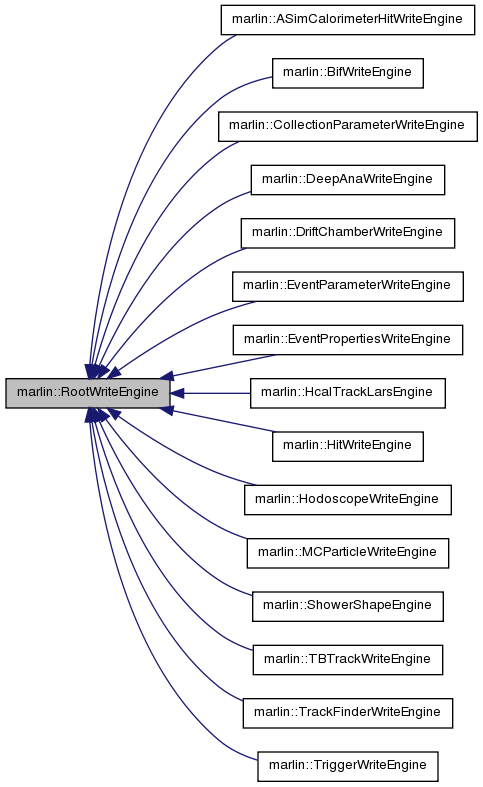
\includegraphics[height=400pt]{classmarlin_1_1RootWriteEngine__inherit__graph}
\end{center}
\end{figure}
Collaboration diagram for marlin::RootWriteEngine:\nopagebreak
\begin{figure}[H]
\begin{center}
\leavevmode
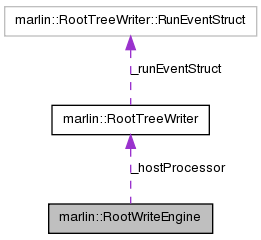
\includegraphics[width=232pt]{classmarlin_1_1RootWriteEngine__coll__graph}
\end{center}
\end{figure}
\subsection*{Public Member Functions}
\begin{DoxyCompactItemize}
\item 
{\bf RootWriteEngine} ({\bf RootTreeWriter} $\ast$host)
\item 
virtual const std::string \& {\bf getEngineName} ()=0
\item 
virtual void {\bf registerParameters} ()=0
\item 
virtual void {\bf registerBranches} (TTree $\ast$)=0
\item 
virtual void {\bf fillVariables} (EVENT::LCEvent $\ast$evt)=0
\end{DoxyCompactItemize}
\subsection*{Protected Attributes}
\begin{DoxyCompactItemize}
\item 
{\bf RootTreeWriter} \& {\bfseries \_\-hostProcessor}\label{classmarlin_1_1RootWriteEngine_ab53e690ff0f758b27f4ef45b87f3d3ce}

\end{DoxyCompactItemize}


\subsection{Detailed Description}
Abstract base class of callback classes for the RootTreeWrite processor Abstract interface for a RootTreeWriter-\/engine. Implement an descendant of this class to add variables to the output tree of the RootTreeWriterProcessor. After that add the new {\itshape engine\/} to the list of writer engines in the \doxyref{RootTreeWriter}{p.}{classmarlin_1_1RootTreeWriter} processor 

Definition at line 29 of file RootWriteEngine.hh.

\subsection{Constructor \& Destructor Documentation}
\index{marlin::RootWriteEngine@{marlin::RootWriteEngine}!RootWriteEngine@{RootWriteEngine}}
\index{RootWriteEngine@{RootWriteEngine}!marlin::RootWriteEngine@{marlin::RootWriteEngine}}
\subsubsection[{RootWriteEngine}]{\setlength{\rightskip}{0pt plus 5cm}marlin::RootWriteEngine::RootWriteEngine ({\bf RootTreeWriter} $\ast$ {\em host})\hspace{0.3cm}{\ttfamily  [inline]}}\label{classmarlin_1_1RootWriteEngine_a9a2f783fbd71d43487cb94feee09210a}
constructor 
\begin{DoxyParams}{Parameters}
\item[\mbox{$\leftarrow$} {\em host}]pointer to the \doxyref{RootTreeWriter}{p.}{classmarlin_1_1RootTreeWriter} processor the constructor of a derived class must pass this pointer to this base class e.g. \begin{DoxyVerb}
    /// SomeeWriteEngine( RootTreeWriter* host ):RootWriteEngine(host),
    ///                                          _engineName("SomeWriteEngine")
    /// {} \end{DoxyVerb}
 \end{DoxyParams}


Definition at line 38 of file RootWriteEngine.hh.

\subsection{Member Function Documentation}
\index{marlin::RootWriteEngine@{marlin::RootWriteEngine}!fillVariables@{fillVariables}}
\index{fillVariables@{fillVariables}!marlin::RootWriteEngine@{marlin::RootWriteEngine}}
\subsubsection[{fillVariables}]{\setlength{\rightskip}{0pt plus 5cm}virtual void marlin::RootWriteEngine::fillVariables (EVENT::LCEvent $\ast$ {\em evt})\hspace{0.3cm}{\ttfamily  [pure virtual]}}\label{classmarlin_1_1RootWriteEngine_ace823bd839cee7e8c8755e60c4cc7134}
Implement this to extract the variables which you want to fill into the {\itshape ROOT\/} tree from the event. Write the value of the variables you want to add to the tree to the member variables, which you registered to the {\itshape ROOT\/} tree. The \doxyref{RootTreeWriter}{p.}{classmarlin_1_1RootTreeWriter} will call TTree::Fill() for you. 
\begin{DoxyParams}{Parameters}
\item[{\em evt}]the current event \end{DoxyParams}


Implemented in {\bf marlin::EventPropertiesWriteEngine} \doxyref{}{p.}{classmarlin_1_1EventPropertiesWriteEngine_abc2305e78939db762a4c83bf669fe952}, {\bf marlin::ASimCalorimeterHitWriteEngine} \doxyref{}{p.}{classmarlin_1_1ASimCalorimeterHitWriteEngine_a23a4c30ce18b277e5dc5150775633d12}, {\bf marlin::BifWriteEngine} \doxyref{}{p.}{classmarlin_1_1BifWriteEngine_a5945f044afb17e832cf63380d3aa4330}, {\bf marlin::CollectionParameterWriteEngine} \doxyref{}{p.}{classmarlin_1_1CollectionParameterWriteEngine_a276cbc4b3fb6a51d52b7ff677cbe60ad}, {\bf marlin::DeepAnaWriteEngine} \doxyref{}{p.}{classmarlin_1_1DeepAnaWriteEngine_a9cf77605dc60b01d00169c80c2df921d}, {\bf marlin::DriftChamberWriteEngine} \doxyref{}{p.}{classmarlin_1_1DriftChamberWriteEngine_ae4ac9d60684437fd6b4d5c3365c0e7ef}, {\bf marlin::EventParameterWriteEngine} \doxyref{}{p.}{classmarlin_1_1EventParameterWriteEngine_ad9ccfdb2f6596c2ae60e6408ad011832}, {\bf marlin::HcalTrackLarsEngine} \doxyref{}{p.}{classmarlin_1_1HcalTrackLarsEngine_a3f7f7a652c8bc019dc0a9b069a2c6fce}, {\bf marlin::HitWriteEngine} \doxyref{}{p.}{classmarlin_1_1HitWriteEngine_a1ee46edbad4693ee7213c153c30dd2d9}, {\bf marlin::HodoscopeWriteEngine} \doxyref{}{p.}{classmarlin_1_1HodoscopeWriteEngine_a4db5d7173b75c3a59d2a8ae86fb0de93}, {\bf marlin::MCParticleWriteEngine} \doxyref{}{p.}{classmarlin_1_1MCParticleWriteEngine_aed3f0a8d52f56cbd1f3f4b93bad9670e}, {\bf marlin::ShowerShapeEngine} \doxyref{}{p.}{classmarlin_1_1ShowerShapeEngine_a02d946fe7bb758c32cff7206109d6882}, {\bf marlin::TBTrackWriteEngine} \doxyref{}{p.}{classmarlin_1_1TBTrackWriteEngine_a5250f4b00f85aabc3be6cff9593dae0f}, {\bf marlin::TrackFinderWriteEngine} \doxyref{}{p.}{classmarlin_1_1TrackFinderWriteEngine_a27566057dc6963c0fb0a5b3f779d6197}, and {\bf marlin::TriggerWriteEngine} \doxyref{}{p.}{classmarlin_1_1TriggerWriteEngine_a6b1216c91a9acbd4f4e09b7d45f3c8f7}.\index{marlin::RootWriteEngine@{marlin::RootWriteEngine}!getEngineName@{getEngineName}}
\index{getEngineName@{getEngineName}!marlin::RootWriteEngine@{marlin::RootWriteEngine}}
\subsubsection[{getEngineName}]{\setlength{\rightskip}{0pt plus 5cm}virtual const std::string\& marlin::RootWriteEngine::getEngineName ()\hspace{0.3cm}{\ttfamily  [pure virtual]}}\label{classmarlin_1_1RootWriteEngine_a31e38120fe60efcb15666fd569ba5862}
Returns the name of the engine to the \doxyref{RootTreeWriter}{p.}{classmarlin_1_1RootTreeWriter} processor. \begin{DoxyReturn}{Returns}
Must return a string with the engine name. 
\end{DoxyReturn}
\begin{Desc}
\item[{\bf Todo}]fixme: should be const, but must be declared const in implementations too. Need to fix all existing engines?!? \end{Desc}


Implemented in {\bf marlin::EventPropertiesWriteEngine} \doxyref{}{p.}{classmarlin_1_1EventPropertiesWriteEngine_ad264b9da6bc60ebd375faa319689941a}, {\bf marlin::ASimCalorimeterHitWriteEngine} \doxyref{}{p.}{classmarlin_1_1ASimCalorimeterHitWriteEngine_a76af2d1c30ce8566f1dcfacf551ab3dc}, {\bf marlin::BifWriteEngine} \doxyref{}{p.}{classmarlin_1_1BifWriteEngine_a82eecc72c7824876b9bb6211d9055e68}, {\bf marlin::CollectionParameterWriteEngine} \doxyref{}{p.}{classmarlin_1_1CollectionParameterWriteEngine_aec77b9403ff1661fd01d714b433157e8}, {\bf marlin::DeepAnaWriteEngine} \doxyref{}{p.}{classmarlin_1_1DeepAnaWriteEngine_a3b67cb94563a6f930a28f71bba8833c1}, {\bf marlin::DriftChamberWriteEngine} \doxyref{}{p.}{classmarlin_1_1DriftChamberWriteEngine_a54c3c6b481d7f957c95dc0b8dd9b9d37}, {\bf marlin::EventParameterWriteEngine} \doxyref{}{p.}{classmarlin_1_1EventParameterWriteEngine_a2a0b15f288547884438d616cba9a6ad0}, {\bf marlin::HcalTrackLarsEngine} \doxyref{}{p.}{classmarlin_1_1HcalTrackLarsEngine_a3d851ed89feec12237cb6c64a14cd54d}, {\bf marlin::HitWriteEngine} \doxyref{}{p.}{classmarlin_1_1HitWriteEngine_a13d17e1b000f55fd5819659426ece2f0}, {\bf marlin::HodoscopeWriteEngine} \doxyref{}{p.}{classmarlin_1_1HodoscopeWriteEngine_a18aa5f3029fd0fc951f8770afdf37f8a}, {\bf marlin::MCParticleWriteEngine} \doxyref{}{p.}{classmarlin_1_1MCParticleWriteEngine_a5cec023911524d85fb491a9a5d702ea0}, {\bf marlin::ShowerShapeEngine} \doxyref{}{p.}{classmarlin_1_1ShowerShapeEngine_ab379dcbe94700542c8a05c302d80231d}, {\bf marlin::TBTrackWriteEngine} \doxyref{}{p.}{classmarlin_1_1TBTrackWriteEngine_ab7ff50302fa10ce40cd78cd87472d1fd}, {\bf marlin::TrackFinderWriteEngine} \doxyref{}{p.}{classmarlin_1_1TrackFinderWriteEngine_a195ec04e9898f5436d1da6ba98886e44}, and {\bf marlin::TriggerWriteEngine} \doxyref{}{p.}{classmarlin_1_1TriggerWriteEngine_a6401f2bbd2a05725c55c851a0e4fcf39}.

Referenced by \_\-\_\-RTW::EngineRegistrar::appendAllEngines().\index{marlin::RootWriteEngine@{marlin::RootWriteEngine}!registerBranches@{registerBranches}}
\index{registerBranches@{registerBranches}!marlin::RootWriteEngine@{marlin::RootWriteEngine}}
\subsubsection[{registerBranches}]{\setlength{\rightskip}{0pt plus 5cm}virtual void marlin::RootWriteEngine::registerBranches (TTree $\ast$)\hspace{0.3cm}{\ttfamily  [pure virtual]}}\label{classmarlin_1_1RootWriteEngine_ad467dc6e73fdd9fd4311f7277fd02a89}
Implement to register local variables to the output tree 
\begin{DoxyParams}{Parameters}
\item[{\em pointer}]to the {\itshape ROOT\/} tree, which the \doxyref{RootTreeWriter}{p.}{classmarlin_1_1RootTreeWriter} processor fills at the end of each event. Usually the implementation looks like \begin{DoxyVerb}
    /// hostTree->Branch("variable",&_variable" ,"variable/F"  );
    /// \end{DoxyVerb}
. But you can add any type of branch you like. \end{DoxyParams}


Implemented in {\bf marlin::EventPropertiesWriteEngine} \doxyref{}{p.}{classmarlin_1_1EventPropertiesWriteEngine_a4c1282d1d34392d66b56de4d7efc6be8}, {\bf marlin::ASimCalorimeterHitWriteEngine} \doxyref{}{p.}{classmarlin_1_1ASimCalorimeterHitWriteEngine_a59a711512fa1cb7f0c3eb39a63af883d}, {\bf marlin::BifWriteEngine} \doxyref{}{p.}{classmarlin_1_1BifWriteEngine_a7589d618bd6113f426333a1aede37855}, {\bf marlin::CollectionParameterWriteEngine} \doxyref{}{p.}{classmarlin_1_1CollectionParameterWriteEngine_afd2c829f35e899f90f881a37aef206f9}, {\bf marlin::DeepAnaWriteEngine} \doxyref{}{p.}{classmarlin_1_1DeepAnaWriteEngine_afa0d65f082b588ef7d61c06aecd9afe4}, {\bf marlin::DriftChamberWriteEngine} \doxyref{}{p.}{classmarlin_1_1DriftChamberWriteEngine_a3b32b9dc07adaa637821917ec5a879a3}, {\bf marlin::EventParameterWriteEngine} \doxyref{}{p.}{classmarlin_1_1EventParameterWriteEngine_ad3a5361c939e7fccab20dc2b334aa33d}, {\bf marlin::HcalTrackLarsEngine} \doxyref{}{p.}{classmarlin_1_1HcalTrackLarsEngine_a5599070ef51668116f4287688f8e62a4}, {\bf marlin::HitWriteEngine} \doxyref{}{p.}{classmarlin_1_1HitWriteEngine_a9de31f39b17a9e782cc7d41d07fce547}, {\bf marlin::HodoscopeWriteEngine} \doxyref{}{p.}{classmarlin_1_1HodoscopeWriteEngine_ac106fb65ad09c7f41975ae5c355da9d2}, {\bf marlin::MCParticleWriteEngine} \doxyref{}{p.}{classmarlin_1_1MCParticleWriteEngine_abc8a55ab829d32228993664ee2fd084e}, {\bf marlin::ShowerShapeEngine} \doxyref{}{p.}{classmarlin_1_1ShowerShapeEngine_aa9b11fb1cee4af0d4dc90a687932c341}, {\bf marlin::TBTrackWriteEngine} \doxyref{}{p.}{classmarlin_1_1TBTrackWriteEngine_a7eeb8a39b0a40bfb13a0d1deb9c143cc}, {\bf marlin::TrackFinderWriteEngine} \doxyref{}{p.}{classmarlin_1_1TrackFinderWriteEngine_aa3fc66248aa14982aacea68e5b67f02e}, and {\bf marlin::TriggerWriteEngine} \doxyref{}{p.}{classmarlin_1_1TriggerWriteEngine_aa83e89d82bb8bc208b02d12d227e2bcb}.\index{marlin::RootWriteEngine@{marlin::RootWriteEngine}!registerParameters@{registerParameters}}
\index{registerParameters@{registerParameters}!marlin::RootWriteEngine@{marlin::RootWriteEngine}}
\subsubsection[{registerParameters}]{\setlength{\rightskip}{0pt plus 5cm}virtual void marlin::RootWriteEngine::registerParameters ()\hspace{0.3cm}{\ttfamily  [pure virtual]}}\label{classmarlin_1_1RootWriteEngine_ae12b70923768043fa5c1438f078c41d3}
Used to register steering parameters. Implement to register {\itshape \doxyref{marlin}{p.}{namespacemarlin}\/} steering file parameters. Use {\itshape \doxyref{marlin}{p.}{namespacemarlin}\/} syntax to register parameters for the calling \doxyref{RootTreeWriter}{p.}{classmarlin_1_1RootTreeWriter} processor.

use \begin{DoxyVerb}
    /// _hostProc.relayRegisterProcessorParameter(...)
    /// _hostProc.relayRegister...()
    /// \end{DoxyVerb}
 instead of {\itshape \doxyref{marlin}{p.}{namespacemarlin}\/} processors \begin{DoxyVerb}register...() \end{DoxyVerb}
 methods 

Implemented in {\bf marlin::EventPropertiesWriteEngine} \doxyref{}{p.}{classmarlin_1_1EventPropertiesWriteEngine_a9394c4461b767c0f763d087988e8c854}, {\bf marlin::ASimCalorimeterHitWriteEngine} \doxyref{}{p.}{classmarlin_1_1ASimCalorimeterHitWriteEngine_a5ad32bcf2f6723033b5a543a715f4d3c}, {\bf marlin::BifWriteEngine} \doxyref{}{p.}{classmarlin_1_1BifWriteEngine_a2f0940793cbb3314fe21843f9bde321b}, {\bf marlin::CollectionParameterWriteEngine} \doxyref{}{p.}{classmarlin_1_1CollectionParameterWriteEngine_ae5bd3085f961a8ecc90272f00886d7d8}, {\bf marlin::DeepAnaWriteEngine} \doxyref{}{p.}{classmarlin_1_1DeepAnaWriteEngine_a757be550fb07212cfbe8cd2a9d6e26be}, {\bf marlin::DriftChamberWriteEngine} \doxyref{}{p.}{classmarlin_1_1DriftChamberWriteEngine_a6632be0ed7f8ef14290e40550d64556c}, {\bf marlin::EventParameterWriteEngine} \doxyref{}{p.}{classmarlin_1_1EventParameterWriteEngine_a05d652e2a9398160729f20aa7d6cdd0d}, {\bf marlin::HcalTrackLarsEngine} \doxyref{}{p.}{classmarlin_1_1HcalTrackLarsEngine_a49bba2b5e26aafb89c9790f35175caae}, {\bf marlin::HitWriteEngine} \doxyref{}{p.}{classmarlin_1_1HitWriteEngine_a54f5c814d074396779ba6d21b2acff6c}, {\bf marlin::HodoscopeWriteEngine} \doxyref{}{p.}{classmarlin_1_1HodoscopeWriteEngine_ad5150110764a1bdd16c8a8eab05ef7bf}, {\bf marlin::MCParticleWriteEngine} \doxyref{}{p.}{classmarlin_1_1MCParticleWriteEngine_a18ac8b6f4d2818bf959ea494d1d17dae}, {\bf marlin::ShowerShapeEngine} \doxyref{}{p.}{classmarlin_1_1ShowerShapeEngine_a861065f4f0a4a91af65a700820cec207}, {\bf marlin::TBTrackWriteEngine} \doxyref{}{p.}{classmarlin_1_1TBTrackWriteEngine_a9ad2d4c87c6a35c554ed34ada4819678}, {\bf marlin::TrackFinderWriteEngine} \doxyref{}{p.}{classmarlin_1_1TrackFinderWriteEngine_a5c154e036f10b5ef6ed6673ec78e7598}, and {\bf marlin::TriggerWriteEngine} \doxyref{}{p.}{classmarlin_1_1TriggerWriteEngine_ae39e2db93985319eb4e8db5c1f6946b1}.

The documentation for this class was generated from the following file:\begin{DoxyCompactItemize}
\item 
RootWriteEngine.hh\end{DoxyCompactItemize}

\section{CALICE::TempSensorBlock Class Reference}
\label{classCALICE_1_1TempSensorBlock}\index{CALICE::TempSensorBlock@{CALICE::TempSensorBlock}}


Class for the Labview Data as acquired by the AHCAL Labview.  


{\ttfamily \#include $<$TempSensorBlock.hh$>$}\subsection*{Public Member Functions}
\begin{DoxyCompactItemize}
\item 
{\bf TempSensorBlock} (int TempSensorNumber, float TempSensorValue)\label{classCALICE_1_1TempSensorBlock_a5577684f2bdde7b3a3f201638f0aaf7a}

\begin{DoxyCompactList}\small\item\em Convenient c'tor. \item\end{DoxyCompactList}\item 
{\bf TempSensorBlock} (LCObject $\ast$obj)\label{classCALICE_1_1TempSensorBlock_ae45af5d892fd90492c15584eb1694190}

\begin{DoxyCompactList}\small\item\em 'Copy constructor' needed to interpret LCCollection read from file/database. \item\end{DoxyCompactList}\item 
virtual {\bf $\sim$TempSensorBlock} ()\label{classCALICE_1_1TempSensorBlock_aededba4f51f50d3056d76a31a97ec1ac}

\begin{DoxyCompactList}\small\item\em Important for memory handling. \item\end{DoxyCompactList}\item 
int {\bfseries GetTempSensorNumber} () const \label{classCALICE_1_1TempSensorBlock_af99dd00f4a3450d25eaa8b2bcb1e2b38}

\item 
float {\bfseries GetTempSensorValue} () const \label{classCALICE_1_1TempSensorBlock_a1485ee33033ab3a99c2ee8d3e5273138}

\item 
void {\bfseries print} (std::ostream \&os, int)\label{classCALICE_1_1TempSensorBlock_af1650378e195b324cfddfa3c2feb9ce6}

\item 
const std::string {\bf getTypeName} () const \label{classCALICE_1_1TempSensorBlock_a00a31b0c70354ed04a4bddc7d62772f3}

\begin{DoxyCompactList}\small\item\em Return the type of the class. \item\end{DoxyCompactList}\item 
const std::string {\bf getDataDescription} () const \label{classCALICE_1_1TempSensorBlock_ab9a8cfa10c171003da2614fb4518b566}

\begin{DoxyCompactList}\small\item\em Return a brief description of the data members. \item\end{DoxyCompactList}\end{DoxyCompactItemize}


\subsection{Detailed Description}
Class for the Labview Data as acquired by the AHCAL Labview. The class reflects that the data are received in the Labview \begin{DoxyAuthor}{Author}
S. Lu DESY Hamburg 
\end{DoxyAuthor}
\begin{DoxyDate}{Date}
Dec 17 2012 
\end{DoxyDate}


Definition at line 23 of file TempSensorBlock.hh.

The documentation for this class was generated from the following file:\begin{DoxyCompactItemize}
\item 
TempSensorBlock.hh\end{DoxyCompactItemize}

\chapter{LABVIEW2LCIO Page Documentation}
\label{todo__todo000001}
 
\begin{DoxyDescription}
\item[Class \doxyref{CALICE::CalibrateAndApplyThreshold}{p.}{classCALICE_1_1CalibrateAndApplyThreshold} ](Re-\/)Verify its applicability for MC after modifs for this release!!!! 
\end{DoxyDescription}

\label{todo__todo000002}
 
\begin{DoxyDescription}
\item[Global \doxyref{CALICE::CellParameter::initADCMemory}{p.}{classCALICE_1_1CellParameter_ad5b4b06d0eb86e98c21d9119fc3a8d30}() ]initialsie with pedestal or zero? 
\end{DoxyDescription}

\label{todo__todo000003}
 
\begin{DoxyDescription}
\item[Class \doxyref{CALICE::Clusteriser}{p.}{classCALICE_1_1Clusteriser} ]: add shower shape criterium, maximum number of tolerated hits 
\end{DoxyDescription}

\label{todo__todo000022}
 
\begin{DoxyDescription}
\item[Class \doxyref{CALICE::CollectionSelector}{p.}{classCALICE_1_1CollectionSelector} ]the simple string should be replaced by regular expressions. 
\end{DoxyDescription}

\label{todo__todo000004}
 
\begin{DoxyDescription}
\item[Class \doxyref{CALICE::MipSelect}{p.}{classCALICE_1_1MipSelect} ]: add shower shape criterium, maximum number of tolerated hits 
\end{DoxyDescription}

\label{todo__todo000012}
 
\begin{DoxyDescription}
\item[Global \doxyref{CALICE::NVector\_\-t::\_\-x}{p.}{classCALICE_1_1NVector__t_a8089ceb5c1305789d489631c1da4913c}\mbox{[}dimension\mbox{]} ]float ? not T ? 

float ? not T ? 
\end{DoxyDescription}

\label{todo__todo000008}
 
\begin{DoxyDescription}
\item[Global \doxyref{CALICE::NVector\_\-t::clear}{p.}{classCALICE_1_1NVector__t_acdcc0e98ea504c04cfc4341269969e5c}() ]: this only works for simple types like int, float, double. 
\end{DoxyDescription}

\label{todo__todo000011}
 
\begin{DoxyDescription}
\item[Global \doxyref{CALICE::NVector\_\-t::data}{p.}{classCALICE_1_1NVector__t_ad523fba7620726c1d58a5b32c8b2d517}() const  ]float ? not T ? 
\end{DoxyDescription}

\label{todo__todo000009}
 
\begin{DoxyDescription}
\item[Global \doxyref{CALICE::NVector\_\-t::operator$\ast$=}{p.}{classCALICE_1_1NVector__t_af177ac27d671789ac8c8d61f257ccd4b}(const float c) ]the argument should not be a float but T ? 
\end{DoxyDescription}

\label{todo__todo000010}
 
\begin{DoxyDescription}
\item[Global \doxyref{CALICE::NVector\_\-t::operator/=}{p.}{classCALICE_1_1NVector__t_ab9758bc6c1ae323e33d25457b1f60993}(const float c) ]the argument should not be a float but T ? 
\end{DoxyDescription}

\label{todo__todo000017}
 
\begin{DoxyDescription}
\item[Global \doxyref{CALICE::SimpleHitSearch::accumulateEventsForPedestalNoiseCalculationWithHitRejectionAndPedestalShiftDetection}{p.}{classCALICE_1_1SimpleHitSearch_a8f264ece7366955c1d742954a28a4d0d}(LCEvent $\ast$evtP) ]useful? 
\end{DoxyDescription}

\label{todo__todo000018}
 
\begin{DoxyDescription}
\item[Global \doxyref{histmgr::FloatHistogram1D::FloatHistogram1D}{p.}{classhistmgr_1_1FloatHistogram1D_a582ec9a1017297a5e56d159aeb18e2b9}(UInt\_\-t id, const \doxyref{HistPar}{p.}{classHistPar} \&binning) ]a name would be better than an ID but a string can not be easily stored in an LCGenericObject 
\end{DoxyDescription}

\label{todo__todo000019}
 
\begin{DoxyDescription}
\item[Global \doxyref{histmgr::FloatHistogram2D::FloatHistogram2D}{p.}{classhistmgr_1_1FloatHistogram2D_a2c53fd92a0a2ffa78589ff109acd1b4b}(UInt\_\-t id, const \doxyref{HistPar}{p.}{classHistPar} \&binning\_\-x, const \doxyref{HistPar}{p.}{classHistPar} \&binning\_\-y) ]a name would be better than an ID but a string can not be easily stored in an LCGenericObject 
\end{DoxyDescription}

\label{todo__todo000020}
 
\begin{DoxyDescription}
\item[Class \doxyref{histmgr::HistMgr::HistogramGroupData\_\-t}{p.}{classhistmgr_1_1HistMgr_1_1HistogramGroupData__t} ]remove \_\-id 
\end{DoxyDescription}

\label{todo__todo000021}
 
\begin{DoxyDescription}
\item[Global \doxyref{histmgr::Profile1D::Profile1D}{p.}{classhistmgr_1_1Profile1D_a89f879d24c7404f5ac2514baa2038a54}(UInt\_\-t id, const \doxyref{HistPar}{p.}{classHistPar} \&binning) ]a name would be better than an ID but a string can not be easily stored in an LCGenericObject 
\end{DoxyDescription}

\label{todo__todo000014}
 
\begin{DoxyDescription}
\item[Class \doxyref{marlin::RunInfoProcessor}{p.}{classmarlin_1_1RunInfoProcessor} ]reduce even more the dependency on hardcoded, god given parameters in the code (valid for many processors)


\end{DoxyDescription}

\label{todo__todo000015}
 
\begin{DoxyDescription}
\item[Global \doxyref{marlin::RunInfoProcessor::handleBeamParameters}{p.}{classmarlin_1_1RunInfoProcessor_a6f3f736a349f45536e3fc13344536950}(LCCDTimeStamp) ]extend scope of function and maybe turn into dedicated class 
\end{DoxyDescription}

\label{todo__todo000016}
 
\begin{DoxyDescription}
\item[Global \doxyref{marlin::RunInfoProcessor::timeCor}{p.}{classmarlin_1_1RunInfoProcessor_a0070ee9315271f15a55ae80c4bb50acc}() ]remove hardcoded times 
\end{DoxyDescription}
\printindex
\end{document}
